
%(BEGIN_QUESTION)
% Copyright 2012, Tony R. Kuphaldt, released under the Creative Commons Attribution License (v 1.0)
% This means you may do almost anything with this work of mine, so long as you give me proper credit

This elevator control system has a problem.  No matter which pushbutton is pressed, the elevator remains ``stuck'' in the full-down position.  The following pictorial diagram shows the wiring of this system, along with the I/O card status lights as they appear with no one pressing any pushbuttons:

$$\includegraphics[width=15.5cm]{i02544x01.eps}$$

Pressing the ``Down'' and ``Up'' pushbuttons, you notice the LEDs for input channels 0 and 3 light up, respectively. 

\vskip 10pt

Based on this information, determine a likely fault causing this elevator to remain stuck at the full-down position.

\underbar{file i02544}
%(END_QUESTION)





%(BEGIN_ANSWER)

There is an electrical fault somewhere in the ``Up'' contactor coil circuit.  Possible faults include:

\begin{itemize}
\item{} Up contactor coil failed open
\item{} Output card channel 3 failed open
\item{} Open wire fault from Up contactor coil to OUT3 terminal
\item{} Open wire fault from terminal 7 to Up contactor coil
\item{} Open wire fault from fuse F3 to VAC 1 terminal
\item{} Fuse F3 blown
\end{itemize}

%(END_ANSWER)





%(BEGIN_NOTES)


%INDEX% PLC, troubleshooting: elevator control system

%(END_NOTES)


